\section{An Overview of NMR Data Analysis}
To gain insights from \ac{NMR} experiments on the chemical system of interest,
extraction of the defining parameters $\bth$ is necessary, though the majority
of \ac{NMR} users are unlikely to think about the process of \ac{NMR} analysis
in this way. For example:
\begin{itemize}
    \item An understanding of the chemical environments of atoms in a molecule
        can be gained by considering the chemical shifts of the various peaks
        in the spectra, which are a proxy for the \ac{FID} frequencies
        $\symbf{f}$.
    \item  The relative stoichiometries\note{does this make sense?} of a
        molecule can be elucidated by inspecting the integrals of spectral
        peaks, which are directly related to the \ac{FID} amplitudes $\bda$
\end{itemize}

\note{
    \begin{itemize}
        \item Typical approach to analysing the data (FT, peak pick, integrate, baseline correction, window functions, zero-filling etc),
        \item Estimation techniques: LP, SVD techniques, iterative techniques (AMARES, VARPRO), Bayesian techniques (CRAFT), ML techniques
    \end{itemize}
}

\subsection{Conventional NMR Analysis}
\label{subsec:nmr-analysis}
The conventional route to interpret \ac{NMR} experiments is to
transform the \ac{FID} into the frequency domain, producing an
\ac{NMR} spectrum. This is achieved through application of the \acfi{FT}:
\begin{subequations}
    \begin{align}
        &\text{Continuous case:} &&\FT(x(t))(F) =  \int_{0}^{\infty} x(t) \exp(
            -2 \pi \iu t F
            ) \mathrm{d} t
            \quad \forall t \in \mathbb{R},\\
        &\text{Discrete case:} &&\FT( \symbf{x} )_n =  \sum_{k=0}^{N-1} x_k \exp \left(
            -\frac{2 \pi \iu k n}{N} \right)
            \quad \forall n \in \lbrace 0, \cdots, N-1 \rbrace.
    \end{align}
\end{subequations}
The \ac{FT} of a continuous exponentially-damped complex sinusoid
takes the form of a \emph{Lorentzian}\footnote{
    An upshot of only possessing data for $t \geq 0$ is
    that the \ac{FT} of an \ac{FID} features a vertical offset,
    such that the baseline does not sit at 0\cite{Tang1994}. This is corrected
    by halving the initial point of the \ac{FID} prior to \ac{FT}.
}:
\begin{subequations}
    \begin{gather}
        s(F) = \FT\left(
            a \exp(\iu \phi) \exp((2 \pi \iu f - \eta)t)
            \right)(F),\\
        s(F) = \frac{a \exp(\iu \phi) }
            {\eta + 2 \pi \iu (f - F)}.
    \end{gather}
\end{subequations}
When $a = \phi = 0$, this function is equivalent to the (unnormalised) \ac{pdf}
of the Cauchy distribution. The \ac{FT} is a linear function, such that the
\ac{FT} of a summation of signals is equivalent to the summation of the
\acp{FT} of each signal. A corollary is that an \ac{NMR} spectrum comprises a
series of Lorentzian ``peaks'', located at the frequencies of all the signals
in the \ac{FID}:
\begin{equation}
    s\left(F\right) = \sum_{m=1}^{M}
    \frac{\amexpphim}
    {\eta_m + 2 \pi \iu (f_m - F)}.
    \label{eq:ft-summation}
\end{equation}
The \ac{FT} is a very attractive means of processing \ac{NMR} data, as it
presents the data in a format which is human-interpretable, with the basic
rules describing how chemical structure is mapped to \ac{NMR} spectral
properties being a fundamental skill that virtually all experimental chemists
require\cite{Hore2015b}. Due to innate properties of the \ac{NMR} experiment,
as well as features arising from analysing a discrete signal, the raw output
from an \ac{NMR} experiment often leads to spectra with undesirable
characteristics without any extra manipulation. Extra processing
steps that are frequently applied to \ac{NMR} data are now outlined, in the
order that they are applied to the data. Note that apodisation and zero filling
are applied to the \ac{FID} (prior to \ac{FT}), while phase correction and
baseline correction are applied to the spectrum (after \ac{FT}).

\begin{figure}
    \centering
    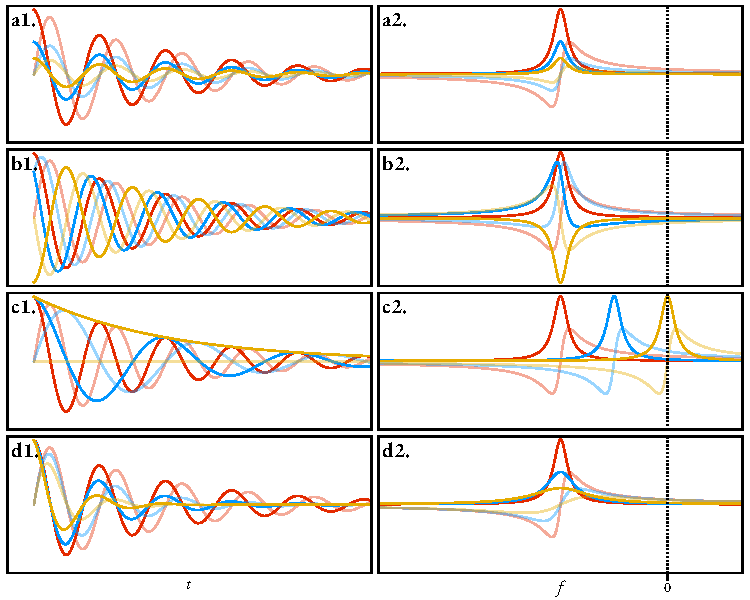
\includegraphics{amp_phase_freq_damp/amp_phase_freq_damp.pdf}
    \caption[
        An illustration of the influence of the four parameters associated
        with an oscillator in both the time-domain nels and Fourier-domain.
    ]{
        An illustration of the influence of the four parameters associated
        with an oscillator in both the time-domain (panels \textbf{a1.} --
        \textbf{d1.}) and Fourier-domain (panels \textbf{a2.} -- \textbf{d2.}).
        The red signal is generated with the same parameters across all panels:
        $a = a_{\text{red}}$, $\phi = 0$, $f = f_{\text{red}}$,  $\eta =
        \eta_{\text{red}}$.  The blue and yellow signals were produced by
        altering one parameter out of the four.
        \textbf{a.} $a_{\text{yellow}} = \nicefrac{1}{2} a_{\text{blue}} =
        \nicefrac{1}{4} a_{\text{red}}$.
        \textbf{b.}
        $\phi_{\text{blue}} = \nicefrac{\pi}{4}$,
        $\phi_{\text{yellow}} = \pi$.
        \textbf{c.}
        $f_{\text{blue}} = \nicefrac{1}{2} f_{\text{red}}$,
        $f_{\text{yellow}} = 0$.
        \textbf{d.}
        $\eta_{\text{blue}} = \nicefrac{1}{2}\eta_{\text{red}}$,
        $\eta_{\text{yellow}} = \nicefrac{1}{4}\eta_{\text{red}}$.
        The real and imaginary components of each signal are plotted, with the
        imaginary component being paler than its real counterpart.
    }
    \label{fig:amp-phase-freq-damp}
\end{figure}

\subsubsection{Apodisation}
Apodisation refers to the process of mutating a signal by multiplying it with a
specified function, often called a \emph{window function}, in order to enhance
a certain property. Apodisation is employed to improve either the sensitivity
or the resolution of the final spectrum, albeit at the cost of worsening the
other feature. There is no such thing as a free lunch after all.

\paragraph{Sensitivity Enhancement} As \iac{FID} progresses with time, the
contributions from the desirable signal ($\bx$) and experimental noise ($\bw$)
becomes more
weighted towards the noise, as spin relaxation phenomena dampen the signal. As
such, multiplying the \ac{FID} with a function which is initially large and
gets progressively smaller with time can be used to enhance the \ac{SNR} of the
\ac{FID}. The most common function to achieve this is the negative exponential
such that a given point is multiplied by $\exp(-\nicefrac{k n}{N - 1})$.
$k$ is referred to as the line broadening factor, since the increased dampening
applied to the signal causes the linewidth of the spectral peaks to increase
(see panel d of Figure \ref{fig:amp-phase-freq-damp}). As such, peaks become
more poorly resolved.

\paragraph{Resolution Enhancement} By contrast, resolution enhancement can be
achieved by applying a window function that artificially reduces the rate of
oscillator decay, by suppressing points that are early in the \ac{FID}. Popular
examples of window functions for resolution enhancement are the Lorentz-Gauss
function, which bestow a sharper, Gaussian shape to the peaks, and the
sine-bell, which is commonly used in multidimensional experiments. Since the
initial points in the \ac{FID} are attenuated these window functions reduce the
sensitivity of the resulting spectra.

By being defined to decay to a sufficiently small value, or $0$, at the end of
the \ac{FID}, window functions are also able to suppress \emph{truncation
artefacts}, which appear when the \ac{FID} still possesses appreciable signal
amplitude at the end of the acquisition period. Truncated \acp{FID} produce
spectra with peaks of a form that is akin to the convolution of the \ac{FT} of
the untruncated \ac{FID}, with the \ac{FT} of a box-function, which takes the
form of a sinc function ($\nicefrac{\sin(x)}{x}$). The resulting artefacts in
spectra are often referred to as \emph{sinc wiggles} for this reason.

\subsubsection{Zero filling}
\note{TODO}

\subsubsection{Phase correction}
The real and imaginary components of \eqref{eq:ft-summation} are as follows:
\begin{subequations}
    \begin{gather}
        \Re(s(F)) = \sum_m
        a_m (\cos(\phi_m) \mathcal{A}_m(F) + \sin(\phi_m) \mathcal{D}_m(F)),\\
        \Im(s(F)) = \sum_m
        a_m (\sin(\phi_m) \mathcal{A}_m(F) - \cos(\phi_m) \mathcal{D}_m(F)),
    \end{gather}
\end{subequations}
where $\mathcal{A}_m$ and  $\mathcal{D}_m$ denote \emph{absorption} and
\emph{dispersion} Lorentzians, respectively:
\begin{subequations}
    \begin{gather}
        \mathcal{A}_m(F) = \frac{\eta_m}{\eta_m^2 + 4 \pi^2 (f_m - F)^2},\\
        \mathcal{D}_m(F) = \frac{2 \pi (f_m - F)}{\eta_m^2 + 4 \pi^2 (f_m - F)^2}.
    \end{gather}
\end{subequations}
As illustrated most clearly in panel c2 of Figure
\ref{fig:amp-phase-freq-damp}, a peak with an absorption lineshape is far more
desirable than one with a dispersion lineshape for two key
reasons: (a) its maximum corresponds to the oscillator frequency, while a
dispersion Lorentzian has a magnitude of $0$ at the oscillator frequency (b)
they decay more rapidly towards $0$ and are therefore more resolved. Generating
a spectrum where all peaks possess absorption Lorentzians is therefore desired,
which is possible if all signal have a phase of \ang{0}, which leads to
\begin{subequations}
    \begin{gather}
        \Re(s(F)) = \sum_m a_m \mathcal{A}_m(F),\label{eq:absorption}\\
        \Im(s(F)) = -\sum_m a_m \mathcal{D}_m(F).\label{eq:dispersion}
    \end{gather}
\end{subequations}
 Fortunately, for the majority of \ac{NMR} experiments\footnote{
     An example of an exception to this rule is when \acl{FS} pulses are applied,
     which generate datasets with quadratic phase behaviour. This is discussed
     in more detail in Section \ref{sec:bbqchili}.
}, the contributing signals possess phases which depend linearly on their
frequencies, i.e.
\begin{equation}
    \phi_m = \Phi_0 + \Phi_1 f_m,
\end{equation}
where $\Phi_0, \in (-\pi, \pi]$ and $\Phi_1 \in \mathbb{R}$ are zero- and
first-order phase terms. A feature of all \ac{NMR} processing platforms is the
ability to perform phase-correction, in which the user determines
$\Phi_0$ and $\Phi_1$ by inspecting the appearance of the spectrum
$\symbf{s}_{\phi}$ for different values of $p_0$ and  $p_1$, according to
\begin{equation}
    s_{\phi,n} = s_n
    \exp\left(\iu \left(p_0 + \frac{p_1 n}{N - 1}\right)\right),
\end{equation}
in an attempt to give all peaks in the spectrum absorption-mode lineshapes.

\subsubsection{Baseline correction}
The \emph{baseline} of an \ac{NMR} spectrum is used to describe regions where
no discernible peaks reside (i.e. only experimental noise exists).
Baseline distortion is used to describe scenarios when the baseline, rather
than exhibiting a flat profile with a moving average of zero, has a distorted
shape instead. There a number of potential causes of baseline distortion,
including acquisition starting at a time $\neq 0$, ``clipping'' of the initial
points due to excessive receiver gain, and ``baseline roll'' due to the
transient response of audio filters\parencites[Section~3.3]{Cavanagh2007}{Tang1994}.
Whatever the cause(s), it is typically the corruption of the initial points in the
\ac{FID} that causes baseline distortion.
It is common to apply baseline correction algorithm after phase correction has
been undertaken to negate any distortion. This involves multiplying
the spectrum with a high-order polynomial function, whose coefficients are
determined by an appropriate algorithm. A popular algorithm
involves the two-step procedure of (a) determining spectral regions which are
part of the baseline (b) fitting the baseline regions to a
polynomial\cite{Dietrich1991,Cobas2006}.

\subsection{Conventional analysis for multidimensional datasets}
\label{subsec:mulitdim}
As for \ac{1D} datasets, it is desirable that multidimensional \ac{NMR} spectra
feature peaks which are (a) frequency discriminated, and (b) comprise pure
absorption-mode lineshapes in each dimension. Frequency discrimination describes
the ability to determine whether a particular resonance is at a frequency which
higher or lower than the frequency of the transmitter, which is in the middle
of the spectral window.

\subsubsection{Amplitude-modulated signals}
It is clear that a cosine modulated signal, given by \eqref{eq:general-fid}
with $D=2$ and $\zeta^{(1)} = \cos(\cdot)$ cannot achieve frequency
discrimination, on account of the relation
\begin{equation}
    \cos\left(2 \pi \fone \tone\right) =
    \tfrac{1}{2} \left(\exp\left(2 \pi \iu \fone \tone \right) + \exp\left(-2 \pi \iu
    \fone \tone \right)\right)
\end{equation}
Performing \ac{FT} on such a signal in both dimensions leads to a spectrum
whose real component comprises two peaks, one at the true resonance frequency
$\left(\fone, \ftwo\right)$, and the other at the mirror-image frequency in the
indirect dimension, $(2\foffone - \fone, \ftwo)$. On top of this, the
peaks possess a mixture of absorption and dispersion character, with the
resultant peak shape often referred to as \emph{phase twist}\cite{Keeler1985}.
A spectrum of this form is presented in panel a of Figure \ref{fig:2d-lineshapes}.
It is possible to generate pure absorption peaks by applying \ac{FT} in the
direct dimension, setting the imaginary component to zero, and finally
applying \ac{FT} in the indirect dimension. The real component of the result
(panel b) is referred to as a \emph{double absorption} spectrum.

To achieve frequency discrimination, it is necessary to also possess the
analogous sine-modulated signal, for which $\zeta^{(1)} = \sin(\cdot)$, as this
in effect achieves quadrature detection in the indirect dimension. For
numerous multidimensional experiments, this can be achieved by repeating the
pulse sequence, with careful adjustments to the phases of particular pulses, in
a process referred to as \emph{phase cycling}\cite[Chapter 11]{Keeler2010}.
Applying the same processing as that which achieved the double absorption
spectrum for the cosine-modulated case generates a spectrum whose imaginary
component features two peaks, but with opposite signs (panel c).
It then becomes possible to generate a frequency discriminated spectrum by
subtracting the sine spectrum from the cosine spectrum (panel d).

\begin{figure}
    \centering
    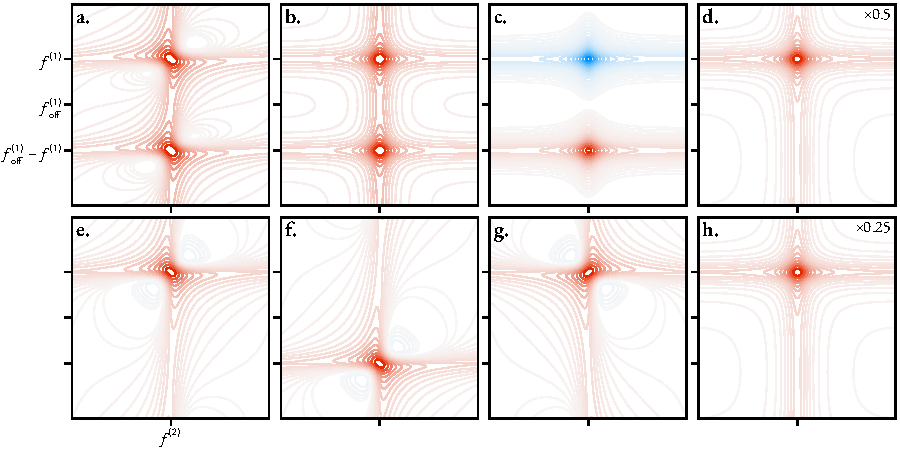
\includegraphics{2d_lineshapes/2d_lineshapes.pdf}
    \caption[
        Spectra acquired from amplitude- and phase-modulated \acs{2D} signals.
    ]{
        Spectra acquired from amplitude- and phase- modulated \acs{2D} signals.
        Red contour lines denote positive values, while blue contours denote
        negative values.
        \textbf{a.} The \ac{FT} of a cosine-modulated \ac{FID}, featuring peaks
        both at the true resonance frequency ($\fone$) and the mirrored
        frequency ($2\foffone - \fone_{\vphantom{off}}$), and with phase-twist lineshapes.
        \textbf{b.} Double-absorption spectrum generated by applying \ac{FT}
        in the direct dimension, setting the imaginary component to zero,
        applying \ac{FT} in the indirect dimension, and retaining the real
        component.
        \textbf{c.} Spectrum acquired with the same processing method as in
        \textbf{b.} but with a sine-modulated \ac{FID}, and with the imaginary
        component retained.
        \textbf{d.} The subtraction of the spectrum in \textbf{c.} from that in
        \textbf{b.} leads to a spectrum with frequency discrimination and a
        pure absorption lineshape.
        \textbf{e.} The \ac{FT} of a positive phase-modulated \ac{FID},
        exhibiting frequency discrimination, but with a phase twist shape.
        \textbf{f.} The \ac{FT} of a negative phase-modulated \ac{FID}.
        \textbf{g.} The spectrum in \textbf{f.} inverted along the indirect
        axis, about $\foffone$.
        \textbf{h.} The summation of \textbf{e.} and \textbf{g.} generates a
        spectrum with an absorption lineshape.
    }
    \label{fig:2d-lineshapes}
\end{figure}

\subsubsection{Phase-modulated signals}

A ``positive'' phase-modulated signal with the form $\zeta^{(1)} = \exp(\iu \cdot)$
(commonly referred to as \emph{hypercomplex}) is frequency-discriminated due to
its quadrature nature. However, direct \ac{FT} of such a signal in both
dimensions leads to a peak with a phase-twist lineshape, with no means of
separating the absorption and dispersion contributions (panel e). Certain pulse
sequences, including \ac{2DJ} spectroscopy\cite{Aue1976,Morris2009} (see
Chapter \ref{chap:cupid}) and
\ac{COSY}\cite{Jeener1971,Jeener2016,Aue1976a} produce hypercomplex datasets,
and the conventional means of processing is simply to display the absolute
value of the spectrum, which while removing the phase twist shapes, produces
peaks with broad wings, due to the influence of the dispersive components. In
scenarios where it is possible, it is desirable to acquire the equivalent
``negative'' signal ($\zeta^{(1)} = \exp(-\iu \cdot)$), whose \ac{FT} leads to
a peak with the same phase twist form, but centered at $2\foffone - \fone$
(panel f). Inverting this spectrum in $\Fone$ (panel g), and summing with the
positive spectrum nullifies the dispersive contribution, generating a spectrum
with an absorption lineshape\cite{Davis1992} (panel h).

\subsection{Estimation Techniques for NMR Analysis}

\subsubsection{\Acl{LP}}

\Ac{LP}\cite{Stephenson1988,Koehl1999} is a procedure which is now widely used
in \ac{NMR} data analysis, often with the intention of (a) propagating the
\ac{FID} further in time in order to reduce the presence of truncation
artefacts and (b) correct the commonly corrupted initial points of the
\ac{FID}, as a means of improving the spectral baseline. The concept of \ac{LP}
stems from the idea that a deterministic signal, such as a \ac{1D} \ac{FID} can
be described as an \ac{AR} process, such that a given sample from the dataset
can be described by a linear combination of an appropriate number $L$ of
previous samples:
\begin{equation}
    y_n = \sum_{l=1}^{L}
    c_l y_{n-l} + e_l
    \label{eq:forward-lp}
\end{equation}
$\forall n \in \lbrace L, L + 1, \cdots, N - 1 \rbrace$, where $L \in
\mathbb{Z}$ defines the order of the linear estimator, and $\symbf{c} \in
\mathbb{R}^{L}$ is a set of \emph{forward} \ac{LP} coefficients. $\symbf{e} \in
\mathbb{R}^L$ is a set of parameters, often called the \emph{innovations},
which account of error in the \ac{LP} model. A datapoint can also be described
by a linear combination of a certain number of subsequent points, using the set
of \emph{backward} \ac{LP} coefficients $\symbf{b} \in \mathbb{R}^L$:
\begin{equation}
    y_n = \sum_{l=1}^{L}
    b_l y_{n+l} + e_l
    \label{eq:backward-lp}
\end{equation}
$\forall n \in \lbrace 0, 1, \cdots, N - L - 1 \rbrace$. Determining
the \ac{LP} coefficients enables the estimation of \ac{FID} values beyond the
data actually acquired ($\none < 0$ and $\none > \None - 1$). It should be noted that
\eqref{eq:forward-lp} and \eqref{eq:backward-lp} are only valid for
\acp{FID} without any corruption from experimental noise. Noisy datasets are
instead an example of an \ac{ARMA} process. Despite this, due to the greater
simplicity of the \ac{AR} model, it is far more common to employ this. The most
common means of performing \ac{LP} is by solving the Yule-Walker
equations\cite{Yule1927,Walker1931},
which describe the relationship between the signal autocorrelation coefficients
and the \ac{LP} coefficients\cite[Section 3.3]{Koehl1999}, with the
Levinson-Durbin algorithm providing an efficient means of solving the
equations\cite{Levinson1946,Durbin1960}.

\note{Stuff below here has been copy-pasted from old document. Will need editing!}
\subsubsection{Signal-Noise Subspace Separation Techniques}

The Linear Prediction with Singular-Value Decomposition was proposed by Kumaresan and Tufts\cite{Kumaresan1982}. The core assumption of the method is that a given data point $y_n$ may be expressed as a linear combination of $L$ previous, or preceeding points:
\begin{equation}
  \begin{split}
    y_n &= b_1 y_{n+1} + b_2 y_{n+2} + \cdots + b_L y_{n+L}\\
    &= b_{-1} y_{n-1} + b_{-2} y_{n-2} + \cdots + b_{-L} y_{n-L}
  \end{split}
\end{equation}
where $b_l$($b_{-l}$), $\ l \in \{ 1, 2, \cdots, L \}$ are the backward(forward) prediction coeffiecients. For the backward prediction case, consider the follwing set of linear equations $\symbf{A} \symbf{b} = - \symbf{h}$:
\begin{equation}
  \label{lineqs}
  \begin{bmatrix}
    y_1^* & y_2^* & \cdots & y_L^*\\
    y_2^* & y_3^* & \cdots & y_{L+1}^*\\
    \vdots & \vdots & \ddots & \vdots\\
    y_{N-L}^* & y_{N-L+1}^* & \cdots & y_{N-1}^*\\
  \end{bmatrix}
  \begin{bmatrix}
    b_1\\
    b_2\\
    \vdots\\
    b_L
  \end{bmatrix}
  = -
  \begin{bmatrix}
    y_0^*\\
    y_1^*\\
    \vdots\\
    y_{N-L-1}^*
  \end{bmatrix}
\end{equation}
This equation can be augmented into the form $\symbf{A}^{\prime} \symbf{b}^{\prime} = \symbf{0}$, with $\symbf{A}^{\prime} = \left[ \symbf{h} \vert \symbf{A} \right]$ and $\symbf{b}^{\prime} = \left[1, \symbf{b}^{\mathrm{T}} \right]^{\mathrm{T}}$. For the noiseless data case (i.e. $y_n = x_n$), any row of $\symbf{A}^{\prime}$ can be written as the linear combination of $J$ linearly independent vectors $\symbf{f}_j,\ j \in \{1, 2, \cdots, J\}$\cite{Kumaresan1983}:
\begin{equation}
  \symbf{f}_j = \left[ 1, z_j^*, \left(z_j^2\right)^*, \cdots, \left(z_j^L\right)^* \right],
\end{equation}
meaning that the rank of $\symbf{A}^{\prime}$ is $J$, provided it posseses at least $J$ rows ($J \leqslant N - L$). The fact that $\symbf{b}^{\prime}$ lies in the null space of $\symbf{A}^{\prime}$ implies that $\symbf{f}_j \symbf{b}^{\prime} = 0$, such that the following holds:
\begin{equation}
  \label{lincom}
  1 + b_1 z_j^* + b_2 \left(z_j^2\right)^* + \cdots + b_L \left(z_j^L\right)^* = 0
\end{equation}
It should be noted that $L$ must satisfy $L \geqslant J$ to ensure the null space of $\symbf{A}^{\prime}$ has at least a dimension of 1.
Eqn. \ref{lincom} leads to a means of deriving the signal poles $z_j$ via polynomial $B(\zeta)$:
\begin{equation}
  B(\zeta) = 1 + b_1 \zeta^{-1} + b_2 \zeta^{-2} + \cdots + b_L \zeta^{-L},
\end{equation}
the zeros of which will occur whenever $\zeta = \left(z_j^{-1}\right)^*,\ j \in \{1, 2, \cdots, J\}$.

Of course, the prediction coefficient vector $\symbf{b}$ still needs to be determined. Eqn. \ref{lineqs} implies that the optimal vector can be determined by simple linear lest squares:
\begin{equation}
  \hat{\symbf{b}} = - \mathbf{A}^+ \symbf{h}.
\end{equation}
However, noise components of the signal will be incorporated into the solution of $\symbf{b}$. To avoid this, $\symbf{A}$ is moved from the signal-noise subspace to the signal subspace via filtration using Singular-Valued Decomposition:
\begin{equation}
  \symbf{A} = \symbf{U}
  \begin{bmatrix}
    \symbf{\Sigma}\\
    \symbf{0}
  \end{bmatrix}
  \symbf{V}^{\dagger} = \sum_{l=1}^R \sigma_l^{\vphantom{\dagger}} \symbf{u}_l^{\vphantom{\dagger}} \symbf{v}_l^{\dagger}
\end{equation}
where $R = \\mathrm{rank}(\symbf{A}) = \min(L, N)$. The matrix $\tilde{\symbf{A}}$ of rank $J$ with the closest relationship to $\symbf{A}$ is a Frobenius norm sense is given by\cite{Cadzow1988}:
\begin{equation}
  \tilde{\symbf{A}} = \sum_{l=1}^J \sigma_l^{\vphantom{\dagger}} \symbf{u}_l^{\vphantom{\dagger}} \symbf{v}_l^{\dagger}.
\end{equation}
Using the following relationship between a matrix's pseudoinverse and its SVD:
\begin{equation}
  \symbf{A}^+ = \symbf{V}
  \begin{bmatrix}
    \symbf{\Sigma}^+\\
    \symbf{0}
  \end{bmatrix}
  \symbf{U}^{\dagger},
\end{equation}
The optimal vector of prediction coeffiecients is determined by:
\begin{equation}
  \hat{\symbf{b}} = - \tilde{\symbf{A}}^+ \symbf{h} = - \sum_{l=1}^J \sigma_l^{-1 \vphantom{\dagger}} \symbf{v}_l^{\vphantom{\dagger}} \left[ \symbf{u}_l^{\dagger} \symbf{h} \right]
\end{equation}
Application: \cite{Barkhuijsen1985}

\note{HSVD, MPM, only gloss over MPM as it is described in detail in Chapter 2}

\subsubsection{Iterative Methods}

The \ac{VARPRO} method is an iterative approach to parameter estimation, developed by Golub and Pereyra\cite{Golub1973}, and applied to NMR signal analysis by van der Veen et al.\cite{VanDerVeen1988}. It relies on minimising the following quantity:
\begin{equation}
  \label{VARPRO_min}
  \hat{\symbf{\theta}} = \argmin_{\symbf{\theta}} \left \lVert \symbf{y} - \symbf{x}(\symbf{\theta}) \right \rVert^2
\end{equation}
The vector $\symbf{x}$ can be expressed in the following format:
\begin{equation}
  \label{VARPRO_Za}
  \symbf{x} =
  \begin{bmatrix}
    z_1^0 & z_2^0 & \cdots & z_J^0\\
    z_1^1 & z_2^1 & \cdots & z_J^1\\
    \vdots & \vdots & \ddots & \vdots\\
    z_1^{N-1} & z_2^{N-1} & \cdots & z_J^{N-1}\\
  \end{bmatrix}
  \begin{bmatrix}
    \alpha_1\\
    \alpha_2\\
    \vdots\\
    \alpha_J
  \end{bmatrix}
  = \symbf{Z}\symbf{\alpha}
\end{equation}
Using Eq. \ref{VARPRO_Za}, Eq. \ref{VARPRO_min} can be re-written as follows:
\begin{equation}
    \hat{\symbf{\theta}} = \argmin_{\symbf{\theta}} \left \lVert \symbf{y} - \symbf{Z}\symbf{\alpha} \right \rVert^2
\end{equation}
The complex amplitudes can be determined analytically as follows:
\begin{equation}
  \label{VARPRO_alpha}
  \hat{\symbf{\alpha}} \approx \left( \symbf{Z}^{\dagger} \symbf{Z} \right)^{-1} \symbf{Z}^{\dagger} \symbf{y} \equiv \symbf{Z}^+ \symbf{y}
\end{equation}
$\symbf{Z}^+$ is the Moore-Penrose pseudoinverse of matrix $\symbf{Z}$\cite{Penrose1955, Strang2018}. The VARPRO method determines the frequencies and damping factors via an iterative minimisation of:
\begin{equation}
  \hat{\left[\symbf{f}^{\mathrm{T}}, \symbf{\eta}^{\mathrm{T}}\right]}^{\mathrm{T}} = \argmin_{\left[\symbf{f}^{\mathrm{T}}, \symbf{\eta}^{\mathrm{T}}\right]} \left \lVert \symbf{y} - \symbf{Z}\symbf{Z}^+\symbf{y} \right \rVert^2
\end{equation}
which is achieved using the Levenberg–Marquardt algorithm\cite{Levenberg1944, Marquardt1963}. The amplitudes and phases are subsequently determined using Eq. \ref{VARPRO_alpha}. This means that the amplitudes and phases do not need initial guesses assocaited with them. Further specifications can be applied to the algorithm, reflecting the spectroscopist's knowledge of the signal under inspection. For example, if it is known that a certain set of resonances constitute a multiplet, the relative frequency differences and amplitudes will be known.

\ac{AMARES}\cite{Vanhamme1997}


\subsubsection{Bayesian Methods}
\ac{CRAFT}\cite{Krishnamurthy2013}
2D\cite{Krishnamurthy2017}
perspective\cite{Krishnamurthy2021}

\subsubsection{Machine Learning Methods}
\cite{Schmid2023}
